% GENERATED by scripts/generate_scaffold.py from the frozen Italian authority.
% Authority SHA-256: BC2D23136027468E9E7BB8DA0E37B4268F38F65AAB6E514FFD8E244BFC4A3032
% CJK fontset: Fandol (bundled by the TeX distribution; exact font hashes are inventoried separately).
\documentclass[11pt]{article}
\usepackage[a4paper,margin=1in]{geometry}
\usepackage{iftex}
\ifPDFTeX
  \PackageError{Bianchi A1 zh scaffold}{Use XeLaTeX or LuaLaTeX}{PDFLaTeX cannot shape the CJK edition.}
\fi
\usepackage[UTF8,scheme=plain,fontset=fandol,heading=false]{ctex}
% SOURCE_DATE_EPOCH fixes dates; xdvipdfmx also needs an explicit trailer ID.
\ifXeTeX
  \special{pdf:trailerid [<BC2D23136027468E9E7BB8DA0E37B426><BC2D23136027468E9E7BB8DA0E37B426>]}
\fi
% Fandol has no small-caps CJK face; declare the already-used regular fallback explicitly.
\ifLuaTeX
  \DeclareFontShape{LTJY3}{FandolSong-Regular(0)}{m}{sc}{<->ssub*FandolSong-Regular(0)/m/n}{}
\fi
\ifXeTeX
  \DeclareFontShape{TU}{FandolSong-Regular(0)}{m}{sc}{<->ssub*FandolSong-Regular(0)/m/n}{}
\fi
\defaultfontfeatures{Ligatures=TeX}
\usepackage{amsmath,amssymb,mathtools}
\usepackage{microtype}
\usepackage{graphicx}
\usepackage{tikz}
\usepackage{enumitem}
\usepackage{longtable,booktabs,array,supertabular}
\usepackage{fancyhdr}
\setlength{\parindent}{1.5em}
\setlength{\parskip}{0.25em}
\setlength{\headheight}{14pt}
% Diagnostic policy: do not suppress badness/overflow warnings.
\emergencystretch=1.5em
\newcommand{\oldquote}{\par\begingroup\leftskip=1.6em\rightskip=0.8em\noindent}
\newcommand{\closeoldquote}{\par\endgroup}
% Number-free, visibly editorial note. It never enters the authorial footnote sequence.
\newcommand{\ednote}[1]{\par\begingroup\small\noindent\textit{【编校注】}#1\par\endgroup}
% Controlled pixel correction: printed p57 distinguishes the original
% coefficient matrix |p_ir| from its transpose |p_ri|; the Italian TeX lost
% that distinction. The accompanying editorial note and ledgers are required.
\providecommand{\pxMatrixOriginal}{\lvert p_{ir}\rvert}
% Controlled pixel correction: printed p69 has a barred initial x with a
% prime, while the Italian TeX drops the prime. The accompanying editorial
% note and PX-0017/PX-0018 ledger evidence are required.
\providecommand{\pxInitialXPrime}{\overline{x}'_i}
% Controlled pixel correction: printed p129 (physical source frame 142)
% has r squared as the leading term of equation (9), while the Italian TeX
% drops the exponent.  The accompanying editorial note and PX-0019/PX-0020
% ledger evidence are required wherever this macro is used.
\providecommand{\pxChFourEquationNineR}{r^2}
% Controlled source-internal correction: printed p207 defines the new
% parameter as u, but the immediately following printed metric and alpha
% both use u_1. The Chinese text renders u_1 only with a visible editorial
% note and PX-0029 through PX-0032 evidence.
\providecommand{\pxChSixUOne}{u_1}
% Controlled source-internal correction: printed p261 repeats bare p,q,r in
% both clauses, although equations (11) determine p',q',r' and only the
% subsequent quadratures determine p,q,r. The visible editorial note and the
% Chapter VIII source-reading ledger are mandatory wherever this macro occurs.
\providecommand{\pxChEightDerivatives}{p',q',r'}
% Controlled scan-proved transcription repair: the inherited Italian TeX
% inserts minus signs that are absent from printed p275 equation (7) and
% printed p288's r-double-prime equation.  This macro is visually empty; the
% formula checker maps it back to the stale minus sign only for structural
% comparison with the frozen working transcription.  PX-0037--PX-0040 and
% SF-0013/SF-0014 are mandatory evidence wherever it occurs.
\providecommand{\pxChNinePrintedPositive}{}
% Printed p288 has D-prime-squared; the frozen Italian working TeX drops the
% prime. This macro renders the scan-proved reading while the checker maps it
% to the stale token stream. Evidence: PX-0039/PX-0040 and SF-0016.
\providecommand{\pxChNineDPrimeSquared}{D'^2}
% Controlled scan-proved transcription repair: printed p410, equation (22),
% has a plus-or-minus sign before every xi term, while the inherited Italian
% and English TeX reduce all three signs to plain plus. The checker maps this macro to the
% stale empty reading only for structural comparison. Chapter XII pixel
% evidence, source finding, and a visible editorial note are mandatory.
\providecommand{\pxChTwelvePlusMinus}{\pm}
% Controlled source-internal correction: printed p428 first gives
% zeta'=zeta/delta^2 but then writes log(zeta'/zeta)=+2 log delta.
% Direct substitution requires the minus sign.  Chinese renders the corrected
% relation only with a visible editorial note and the Chapter XIII pixel
% evidence; the formula lock maps this macro back to the literal printed plus.
\providecommand{\pxChThirteenDistanceLog}{-2\log\delta}
% Controlled source-internal correction: printed p440 describes n independent
% variables u_r but gives the impossible isolated range r=1,2,4.  Chinese
% renders the general range r=1,2,...,n with a visible editorial note; the
% formula lock maps this macro back to the literal printed range.
\providecommand{\pxChThirteenIndependentRange}{r=1,2,\ldots,n}
\providecommand{\pxChThirteenUnequalTorsionMagnitude}{\pm\frac1R}
% Controlled scan-proved transcription repair: printed p414, equation (2*),
% has the second-kind four-index symbols {rk,ih} and {rk,ik}, followed by
% K a_{ri}.  The inherited Italian/English digital layers instead have
% [ri,ih], [ri,ik], and K a_{rk}.  These macros render the source pixels in
% Chinese; the formula checker maps them to the stale inherited stream only
% to localize the already-documented defect. Evidence: SF-0045, PX-0117/0118.
\providecommand{\pxChThirteenSecondKindZeroSymbol}{\chrfour{rk}{ih}}
\providecommand{\pxChThirteenSecondKindCurvatureSymbol}{\chrfour{rk}{ik}}
\providecommand{\pxChThirteenSecondKindCurvatureCoefficient}{a_{ri}}
% Controlled scan-proved repair: printed p483 clearly names the representative
% Euclidean space S'_n, while the frozen Italian TeX drops the prime.
\providecommand{\pxChFourteenRepresentativeSpace}{S'_n}
% Controlled source-internal correction: on printed p483 the tangent-hyperplane
% equations are printed with r=0,...,n, although the hypersurface has only the
% parameters u_1,...,u_{n-1}. The surrounding definitions and all subsequent
% formulae force the corrected range r=1,...,n-1.
\providecommand{\pxChFourteenTangentRange}{(r=1,2,\ldots,n-1)}
% Controlled source-internal correction: printed p493 writes K although this
% paragraph and equation (VIII) define the ambient curvature as K_0. The
% Chinese reading uses K_0 with a visible editorial note; the structural
% checker maps this macro back to the literal printed/Italian token K.
\providecommand{\pxChFourteenAmbientK}{K_0}
% Controlled scan-proved transcription repair: printed p493 has the scalar
% product of the nu-components with coordinate indices lambda and lambda'.
% The inherited Italian/English TeX instead substitutes x_lambda/u_r and
% x_lambda'/u_s. The Chinese formula follows the source pixels.
\providecommand{\pxChFourteenEqFortyDerivativeProduct}{%
  \frac{\partial x_\nu}{\partial u_\lambda}%
  \frac{\partial x_\nu}{\partial u_{\lambda'}}}
% Controlled scan-proved transcription repair: printed p494 sums over
% lambda' and gives the two-index Kronecker delta epsilon_{lambda mu'}.
% The inherited TeX changes both the summation index and epsilon subscript.
\providecommand{\pxChFourteenKroneckerIdentity}{%
  \sum_{\lambda'}b_{\lambda\lambda'}B_{\lambda'\mu'}%
  =\varepsilon_{\lambda\mu'}}
% Target-only line-breaking controls for the long p492--494 displays. The
% formula checker removes these macro names before structural comparison, so
% line fitting cannot alter the mathematical token stream.
\providecommand{\pxChFourteenDisplayBreak}{\\[-0.15em]&\qquad{}}
\providecommand{\pxChFourteenAlignBegin}{\begin{aligned}}
\providecommand{\pxChFourteenAlignMark}{&}
\providecommand{\pxChFourteenAlignEnd}{\end{aligned}}
% Controlled scan-proved transcription repairs on printed pp494 and 496.
% The source has explicit nu-summation signs in both expressions; the frozen
% Italian/English TeX reduces them to a bare S and also drops the nu on xi in
% the Enneper calculation.
\providecommand{\pxChFourteenEllipticConjugacySum}{%
  \sum_\nu dx_\nu\,\delta\xi_\nu=0}
\providecommand{\pxChFourteenEnneperSum}{%
  \sum_\nu\frac{d\xi_\nu^2}{ds^2}}
% Printed p494 has delta xi_i in the hyperbolic conjugacy equation; the
% inherited TeX silently substitutes delta x_i.
\providecommand{\pxChFourteenHyperbolicDeltaXi}{\delta\xi_i}
% Controlled scan-proved transcription repair: printed p500 places a bar
% over xi_nu in the displayed tangent-plane coordinate. The inherited
% Italian and English TeX omit the bar despite naming \overline{xi} in prose.
\providecommand{\pxChFourteenBarredTangentCoordinate}{\overline{\xi}_\nu}
% Controlled scan-proved transcription repair: printed p507 uses the
% u-derivative for the generating tangent in all three relevant formulae.
% The inherited Italian and English TeX substitute v. The Chinese edition
% renders u; the formula lock maps this macro back to stale v only for
% structural comparison. Evidence is retained in dense_gates_s219.
\providecommand{\pxChFourteenGeneratingTangentParameter}{u}
% Controlled scan-proved transcription repair: printed p508 distinguishes
% the ruled-surface line element as ds'^2 in both displays. The inherited
% Italian and English TeX drop the prime. Chinese follows the scan pixels.
\providecommand{\pxChFourteenRuledLineElement}{ds'^2}
% Controlled source-internal corrections proved from printed pp493 and 495:
% both displayed quadratic forms repeat D' on dv^2 although the second
% fundamental form and the local component calculations require D''.
\providecommand{\pxChFourteenSecondFormDvCoefficient}{D''}
% Controlled source-internal correction on printed p503. Completing the
% immediately preceding theta equation gives h^4 R^2 - 4c^2, and the next
% printed integral independently uses the same h^4 term.
\providecommand{\pxChFourteenCompletedSquareConstant}{(h^4R^2-4c^2)}
% Controlled source-internal correction on printed p512. The printed left
% ratio reverses D_1 and D'_1 even though both displayed zero coefficients
% occupy the primed middle position.
\providecommand{\pxChFourteenCoefficientRatio}{D_1:D'_1:D''_1=D:D':D''}
% The printed index on p520 and the §101 heading/body all read infinity cubed;
% the frozen Italian index TeX alone mistranscribes that entry as infinity one.
% Chinese follows the scan. The structural checker maps this controlled macro
% back only when comparing with the stale Italian index token stream.
\providecommand{\pxIndexConstantCurvatureSelfApplicability}{\infty^3}
\newcommand{\diff}{\mathrm{d}}
\newcommand{\detmat}[1]{\left|\begin{matrix}#1\end{matrix}\right|}
% Added in p0505-p0543 final tranche for source-style two-row Christoffel symbols.
\providecommand{\Ctwo}[2]{\left\{\begin{matrix}#1\\#2\end{matrix}\right\}}
\providecommand{\cotg}{\operatorname{cotg}}

\pagestyle{plain}
\allowdisplaybreaks

% Source-style footnote marks: preserve scan-visible parenthesized markers.
\makeatletter
\newcommand{\srcfnmark}[1]{\textsuperscript{(#1)}}
\newcommand{\srcfntext}[2]{%
  \begingroup
  \def\@thefnmark{(#1)}%
  \@footnotetext{#2}%
  \endgroup
}
\newcommand{\srcfn}[2]{%
  \begingroup
  \def\@thefnmark{(#1)}%
  \@footnotemark
  \@footnotetext{#2}%
  \endgroup
}
\providecommand{\scanrestoredsrcfnmark}[1]{\srcfnmark{#1}}
\providecommand{\scanrestoredsrcfntext}[2]{\srcfntext{#1}{#2}}
\makeatother


\DeclareMathOperator{\sen}{sen}
\DeclareMathOperator{\tg}{tg}

\DeclareMathOperator{\senh}{senh}
\DeclareMathOperator{\cn}{cn}
\DeclareMathOperator{\sn}{sn}
\DeclareMathOperator{\dn}{dn}
\DeclareMathOperator{\arc}{arc}
\DeclareMathOperator{\sett}{sett}
\DeclareMathOperator{\tgh}{tgh}



\newcommand{\chr}[3]{\left\{\begin{matrix}#1#2\\#3\end{matrix}\right\}}
\newcommand{\chrsq}[3]{\left[\begin{matrix}#1#2\\#3\end{matrix}\right]}

% Current-slice two-row Christoffel symbol macros, kept distinct from the older three-argument macros.
\providecommand{\chrB}[2]{\left\{\begin{matrix}#1\\#2\end{matrix}\right\}}
\providecommand{\chrsqB}[2]{\left[\begin{matrix}#1\\#2\end{matrix}\right]}

\newcommand{\chrfour}[2]{\left\{#1,#2\right\}}
\newcommand{\bigdet}[1]{\left|\begin{matrix}#1\end{matrix}\right|}
\newcommand{\dd}{\,d}

\renewcommand{\srcfnmark}[1]{\ifmmode{}^{(#1)}\else\textsuperscript{(#1)}\fi}

% Additional operators encountered in source pdfpages 0281-0312.
\providecommand{\tgh}{\operatorname{tgh}}
\providecommand{\tang}{\operatorname{tang}}
\providecommand{\tangh}{\operatorname{tangh}}
\providecommand{\coth}{\operatorname{coth}}

\newcommand{\figseven}{%
\begin{center}\includegraphics[width=.34\textwidth]{assets/ch12_figures/Luigi_Bianchi_Geometria_differenziale_Figura_7_facsimile.png}\end{center}}
\newcommand{\figsevena}{%
\begin{center}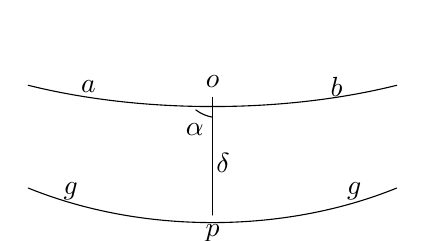
\begin{tikzpicture}[scale=0.9,line cap=round,line join=round]
\draw (-2.6,.65) .. controls (-1,.25) and (1,.25) .. (2.6,.65);
\draw (-2.6,-.8) .. controls (-1,-1.45) and (1,-1.45) .. (2.6,-.8);
\draw (0,.48)--(0,-1.18); \node[above] at (0,.48) {$o$}; \node[below] at (0,-1.18) {$p$};
\node at (-1.75,.63) {$a$}; \node at (1.75,.63) {$b$}; \node at (-2.0,-.85) {$g$}; \node at (2.0,-.85) {$g$};
\draw (0,.2) arc (260:233:.55); \node at (-.25,.03) {$\alpha$}; \node at (.15,-.45) {$\delta$};
\end{tikzpicture}\\[-.2em]{\small Fig. 7a.}\end{center}}
\newcommand{\figeight}{%
\begin{center}\includegraphics[width=.33\textwidth]{assets/ch12_figures/Luigi_Bianchi_Geometria_differenziale_Figura_8_facsimile.png}\end{center}}
\newcommand{\fignine}{%
\begin{center}\includegraphics[width=.43\textwidth]{assets/ch12_figures/Luigi_Bianchi_Geometria_differenziale_Figura_9_facsimile.png}\end{center}}


% compatibility shims for p0409--0440 continuation
\providecommand{\sen}{\operatorname{sen}}
\providecommand{\tg}{\operatorname{tg}}
\providecommand{\senh}{\operatorname{senh}}
\providecommand{\tgh}{\operatorname{tgh}}
\providecommand{\cotgh}{\operatorname{cotgh}}
\providecommand{\ang}{\operatorname{ang}}
\providecommand{\grad}{\operatorname{grad}}
\providecommand{\chrB}[2]{\left\{\begin{matrix}#1\\#2\end{matrix}\right\}}
\providecommand{\chrsqB}[2]{\left[\begin{matrix}#1\\#2\end{matrix}\right]}
